% !TEX root = tnnls_relation_gait.tex

\ifx\allfiles\undefined
    % !TEX root = tnnls_relation_gait.tex

%% bare_jrnl.tex
%% V1.4b
%% 2015/08/26
%% by Michael Shell
%% see http://www.michaelshell.org/
%% for current contact information.
%%
%% This is a skeleton file demonstrating the use of IEEEtran.cls
%% (requires IEEEtran.cls version 1.8b or later) with an IEEE
%% journal paper.
%%
%% Support sites:
%% http://www.michaelshell.org/tex/ieeetran/
%% http://www.ctan.org/pkg/ieeetran
%% and
%% http://www.ieee.org/

%%*************************************************************************
%% Legal Notice:
%% This code is offered as-is without any warranty either expressed or
%% implied; without even the implied warranty of MERCHANTABILITY or
%% FITNESS FOR A PARTICULAR PURPOSE!
%% User assumes all risk.
%% In no event shall the IEEE or any contributor to this code be liable for
%% any damages or losses, including, but not limited to, incidental,
%% consequential, or any other damages, resulting from the use or misuse
%% of any information contained here.
%%
%% All comments are the opinions of their respective authors and are not
%% necessarily endorsed by the IEEE.
%%
%% This work is distributed under the LaTeX Project Public License (LPPL)
%% ( http://www.latex-project.org/ ) version 1.3, and may be freely used,
%% distributed and modified. A copy of the LPPL, version 1.3, is included
%% in the base LaTeX documentation of all distributions of LaTeX released
%% 2003/12/01 or later.
%% Retain all contribution notices and credits.
%% ** Modified files should be clearly indicated as such, including  **
%% ** renaming them and changing author support contact information. **
%%*************************************************************************


% *** Authors should verify (and, if needed, correct) their LaTeX system  ***
% *** with the testflow diagnostic prior to trusting their LaTeX platform ***
% *** with production work. The IEEE's font choices and paper sizes can   ***
% *** trigger bugs that do not appear when using other class files.       ***                          ***
% The testflow support page is at:
% http://www.michaelshell.org/tex/testflow/

\documentclass[journal]{IEEEtran}
%
% If IEEEtran.cls has not been installed into the LaTeX system files,
% manually specify the path to it like:
% \documentclass[journal]{../sty/IEEEtran}

% Some very useful LaTeX packages include:
% (uncomment the ones you want to load)

% *** MISC UTILITY PACKAGES ***
%
%\usepackage{ifpdf}
% Heiko Oberdiek's ifpdf.sty is very useful if you need conditional
% compilation based on whether the output is pdf or dvi.
% usage:
% \ifpdf
%   % pdf code
% \else
%   % dvi code
% \fi
% The latest version of ifpdf.sty can be obtained from:
% http://www.ctan.org/pkg/ifpdf
% Also, note that IEEEtran.cls V1.7 and later provides a builtin
% \ifCLASSINFOpdf conditional that works the same way.
% When switching from latex to pdflatex and vice-versa, the compiler may
% have to be run twice to clear warning/error messages.

% *** CITATION PACKAGES ***

\usepackage{tabularx}
\usepackage{longtable}
\usepackage{threeparttable}
\usepackage{cite}

% cite.sty was written by Donald Arseneau
% V1.6 and later of IEEEtran pre-defines the format of the cite.sty package
% \cite{} output to follow that of the IEEE. Loading the cite package will
% result in citation numbers being automatically sorted and properly
% "compressed/ranged". e.g., [1], [9], [2], [7], [5], [6] without using
% cite.sty will become [1], [2], [5]--[7], [9] using cite.sty. cite.sty's
% \cite will automatically add leading space, if needed. Use cite.sty's
% noadjust option (cite.sty V3.8 and later) if you want to turn this off
% such as if a citation ever needs to be enclosed in parenthesis.
% cite.sty is already installed on most LaTeX systems. Be sure and use
% version 5.0 (2009-03-20) and later if using hyperref.sty.
% The latest version can be obtained at:
% http://www.ctan.org/pkg/cite
% The documentation is contained in the cite.sty file itself.

% *** GRAPHICS RELATED PACKAGES ***
%
\usepackage[pdftex]{graphicx}
\usepackage{rotating}
\ifCLASSINFOpdf
  % \usepackage[pdftex]{graphicx}
  % declare the path(s) where your graphic files are
  % \graphicspath{{../pdf/}{../jpeg/}}
  % and their extensions so you won't have to specify these with
  % every instance of \includegraphics
  % \DeclareGraphicsExtensions{.pdf,.jpeg,.png}
\else
  % or other class option (dvipsone, dvipdf, if not using dvips). graphicx
  % will default to the driver specified in the system graphics.cfg if no
  % driver is specified.
  % \usepackage[dvips]{graphicx}
  % declare the path(s) where your graphic files are
  % \graphicspath{{../eps/}}
  % and their extensions so you won't have to specify these with
  % every instance of \includegraphics
  % \DeclareGraphicsExtensions{.eps}
\fi
% graphicx was written by David Carlisle and Sebastian Rahtz. It is
% required if you want graphics, photos, etc. graphicx.sty is already
% installed on most LaTeX systems. The latest version and documentation
% can be obtained at:
% http://www.ctan.org/pkg/graphicx
% Another good source of documentation is "Using Imported Graphics in
% LaTeX2e" by Keith Reckdahl which can be found at:
% http://www.ctan.org/pkg/epslatex
%
% latex, and pdflatex in dvi mode, support graphics in encapsulated
% postscript (.eps) format. pdflatex in pdf mode supports graphics
% in .pdf, .jpeg, .png and .mps (metapost) formats. Users should ensure
% that all non-photo figures use a vector format (.eps, .pdf, .mps) and
% not a bitmapped formats (.jpeg, .png). The IEEE frowns on bitmapped formats
% which can result in "jaggedy"/blurry rendering of lines and letters as
% well as large increases in file sizes.
%
% You can find documentation about the pdfTeX application at:
% http://www.tug.org/applications/pdftex

% *** MATH PACKAGES ***
%
\usepackage{amsmath}
% A popular package from the American Mathematical Society that provides
% many useful and powerful commands for dealing with mathematics.
%
% Note that the amsmath package sets \interdisplaylinepenalty to 10000
% thus preventing page breaks from occurring within multiline equations. Use:
%\interdisplaylinepenalty=2500
% after loading amsmath to restore such page breaks as IEEEtran.cls normally
% does. amsmath.sty is already installed on most LaTeX systems. The latest
% version and documentation can be obtained at:
% http://www.ctan.org/pkg/amsmath

% *** SPECIALIZED LIST PACKAGES ***
%
\usepackage{algorithmic}
% algorithmic.sty was written by Peter Williams and Rogerio Brito.
% This package provides an algorithmic environment fo describing algorithms.
% You can use the algorithmic environment in-text or within a figure
% environment to provide for a floating algorithm. Do NOT use the algorithm
% floating environment provided by algorithm.sty (by the same authors) or
% algorithm2e.sty (by Christophe Fiorio) as the IEEE does not use dedicated
% algorithm float types and packages that provide these will not provide
% correct IEEE style captions. The latest version and documentation of
% algorithmic.sty can be obtained at:
% http://www.ctan.org/pkg/algorithms
% Also of interest may be the (relatively newer and more customizable)
% algorithmicx.sty package by Szasz Janos:
% http://www.ctan.org/pkg/algorithmicx

% *** ALIGNMENT PACKAGES ***
%
\usepackage{array}
% Frank Mittelbach's and David Carlisle's array.sty patches and improves
% the standard LaTeX2e array and tabular environments to provide better
% appearance and additional user controls. As the default LaTeX2e table
% generation code is lacking to the point of almost being broken with
% respect to the quality of the end results, all users are strongly
% advised to use an enhanced (at the very least that provided by array.sty)
% set of table tools. array.sty is already installed on most systems. The
% latest version and documentation can be obtained at:
% http://www.ctan.org/pkg/array

% IEEEtran contains the IEEEeqnarray family of commands that can be used to
% generate multiline equations as well as matrices, tables, etc., of high
% quality.

% *** SUBFIGURE PACKAGES ***
\usepackage[caption=false,font=footnotesize]{subfig}
%\ifCLASSOPTIONcompsoc
%  \usepackage[caption=false,font=normalsize,labelfont=sf,textfont=sf]{subfig}
%\else
%  \usepackage[caption=false,font=footnotesize]{subfig}
%\fi
% subfig.sty, written by Steven Douglas Cochran, is the modern replacement
% for subfigure.sty, the latter of which is no longer maintained and is
% incompatible with some LaTeX packages including fixltx2e. However,
% subfig.sty requires and automatically loads Axel Sommerfeldt's caption.sty
% which will override IEEEtran.cls' handling of captions and this will result
% in non-IEEE style figure/table captions. To prevent this problem, be sure
% and invoke subfig.sty's "caption=false" package option (available since
% subfig.sty version 1.3, 2005/06/28) as this is will preserve IEEEtran.cls
% handling of captions.
% Note that the Computer Society format requires a larger sans serif font
% than the serif footnote size font used in traditional IEEE formatting
% and thus the need to invoke different subfig.sty package options depending
% on whether compsoc mode has been enabled.
%
% The latest version and documentation of subfig.sty can be obtained at:
% http://www.ctan.org/pkg/subfig

% *** FLOAT PACKAGES ***
%
%\usepackage{fixltx2e}
% fixltx2e, the successor to the earlier fix2col.sty, was written by
% Frank Mittelbach and David Carlisle. This package corrects a few problems
% in the LaTeX2e kernel, the most notable of which is that in current
% LaTeX2e releases, the ordering of single and double column floats is not
% guaranteed to be preserved. Thus, an unpatched LaTeX2e can allow a
% single column figure to be placed prior to an earlier double column
% figure.
% Be aware that LaTeX2e kernels dated 2015 and later have fixltx2e.sty's
% corrections already built into the system in which case a warning will
% be issued if an attempt is made to load fixltx2e.sty as it is no longer
% needed.
% The latest version and documentation can be found at:
% http://www.ctan.org/pkg/fixltx2e

%\usepackage{stfloats}
% stfloats.sty was written by Sigitas Tolusis. This package gives LaTeX2e
% the ability to do double column floats at the bottom of the page as well
% as the top. (e.g., "\begin{figure*}[!b]" is not normally possible in
% LaTeX2e). It also provides a command:
%\fnbelowfloat
% to enable the placement of footnotes below bottom floats (the standard
% LaTeX2e kernel puts them above bottom floats). This is an invasive package
% which rewrites many portions of the LaTeX2e float routines. It may not work
% with other packages that modify the LaTeX2e float routines. The latest
% version and documentation can be obtained at:
% http://www.ctan.org/pkg/stfloats
% Do not use the stfloats baselinefloat ability as the IEEE does not allow
% \baselineskip to stretch. Authors submitting work to the IEEE should note
% that the IEEE rarely uses double column equations and that authors should try
% to avoid such use. Do not be tempted to use the cuted.sty or midfloat.sty
% packages (also by Sigitas Tolusis) as the IEEE does not format its papers in
% such ways.
% Do not attempt to use stfloats with fixltx2e as they are incompatible.
% Instead, use Morten Hogholm'a dblfloatfix which combines the features
% of both fixltx2e and stfloats:
%
% \usepackage{dblfloatfix}
% The latest version can be found at:
% http://www.ctan.org/pkg/dblfloatfix

%\ifCLASSOPTIONcaptionsoff
%  \usepackage[nomarkers]{endfloat}
% \let\MYoriglatexcaption\caption
% \renewcommand{\caption}[2][\relax]{\MYoriglatexcaption[#2]{#2}}
%\fi
% endfloat.sty was written by James Darrell McCauley, Jeff Goldberg and
% Axel Sommerfeldt. This package may be useful when used in conjunction with
% IEEEtran.cls'  captionsoff option. Some IEEE journals/societies require that
% submissions have lists of figures/tables at the end of the paper and that
% figures/tables without any captions are placed on a page by themselves at
% the end of the document. If needed, the draftcls IEEEtran class option or
% \CLASSINPUTbaselinestretch interface can be used to increase the line
% spacing as well. Be sure and use the nomarkers option of endfloat to
% prevent endfloat from "marking" where the figures would have been placed
% in the text. The two hack lines of code above are a slight modification of
% that suggested by in the endfloat docs (section 8.4.1) to ensure that
% the full captions always appear in the list of figures/tables - even if
% the user used the short optional argument of \caption[]{}.
% IEEE papers do not typically make use of \caption[]'s optional argument,
% so this should not be an issue. A similar trick can be used to disable
% captions of packages such as subfig.sty that lack options to turn off
% the subcaptions:
% For subfig.sty:
% \let\MYorigsubfloat\subfloat
% \renewcommand{\subfloat}[2][\relax]{\MYorigsubfloat[]{#2}}
% However, the above trick will not work if both optional arguments of
% the \subfloat command are used. Furthermore, there needs to be a
% description of each subfigure *somewhere* and endfloat does not add
% subfigure captions to its list of figures. Thus, the best approach is to
% avoid the use of subfigure captions (many IEEE journals avoid them anyway)
% and instead reference/explain all the subfigures within the main caption.
% The latest version of endfloat.sty and its documentation can obtained at:
% http://www.ctan.org/pkg/endfloat
%
% The IEEEtran \ifCLASSOPTIONcaptionsoff conditional can also be used
% later in the document, say, to conditionally put the References on a
% page by themselves.

% *** PDF, URL AND HYPERLINK PACKAGES ***
%
\usepackage{url}
% url.sty was written by Donald Arseneau. It provides better support for
% handling and breaking URLs. url.sty is already installed on most LaTeX
% systems. The latest version and documentation can be obtained at:
% http://www.ctan.org/pkg/url
% Basically, \url{my_url_here}.

% *** Do not adjust lengths that control margins, column widths, etc. ***
% *** Do not use packages that alter fonts (such as pslatex).         ***
% There should be no need to do such things with IEEEtran.cls V1.6 and later.
% (Unless specifically asked to do so by the journal or conference you plan
% to submit to, of course. )

% correct bad hyphenation here
% \hyphenation{op-tical net-works semi-conduc-tor}
\usepackage{enumerate}
\usepackage{multirow}
\usepackage{color}
\usepackage{threeparttable}
\usepackage{booktabs}
\newcommand{\minus}{\scalebox{0.75}[1.0]{$-$}}
\newcommand{\bftab}[1]{{\fontseries{b}\selectfont#1}}
\newcommand{\tabincell}[2]{\begin{tabular}{@{}#1@{}}#2\end{tabular}}
\newcommand{\etal}{\textit{et al}.}
\newcommand{\ie}{\textit{i.e.}}
\newcommand{\eg}{\textit{e.g.}}
\newcommand{\wrt}{\textit{w.r.t.}}
\newcommand{\vs}{\textit{vs.}}


\begin{document}
%
% paper title
% Titles are generally capitalized except for words such as a, an, and, as,
% at, but, by, for, in, nor, of, on, or, the, to and up, which are usually
% not capitalized unless they are the first or last word of the title.
% Linebreaks \\ can be used within to get better formatting as desired.
% Do not put math or special symbols in the title.
%\title{The Application and Research of Multi-modal Data in Auxiliary Diagnosis of Depression: A Survey
%}
\title{ Auxiliary Diagnosis of Depression Based on Multi-modal Data: A Survey
}
%%
%%
%% author names and IEEE memberships
%% note positions of commas and nonbreaking spaces ( ~ ) LaTeX will not break
%% a structure at a ~ so this keeps an author's name from being broken across
%% two lines.
%% use \thanks{} to gain access to the first footnote area
%% a separate \thanks must be used for each paragraph as LaTeX2e's \thanks
%% was not built to handle multiple paragraphs
%%
%
%\author{Saihui~Hou,
%	Xu~Liu,
%	Chunshui~Cao,
%	and~Yongzhen~Huang$^*$% <-this % stops a space
%	\thanks{$^*$ indicates the corresponding author.}% <-this % stops a space
%    \thanks{Saihui Hou and Yongzhen Huang is with School of Artificial Intelligence, Beijing Normal University, Beijing 100875, China. (Email: housaihui@bnu.edu.cn, huangyongzhen@bnu.edu.cn)}
%	\thanks{Xu Liu and Chunshui Cao are with Watrix Technology Limited Co. Ltd, Beijing 100088, China. (Email: xu.liu@watrix.ai, chunshuicao@watrix.ai)}
%    \thanks{This work is partially supported by the Fundamental Research Funds for the Central Universities.}
%    % \thanks{E-mail: housaihui@bnu.edu.cn, xu.liu@watrix.ai, chunshuicao@watrix.ai, huangyongzhen@bnu.edu.cn}
%	% \thanks{Manuscript received April 19, 2005; revised August 26, 2015.}
%}
%
%% note the % following the last \IEEEmembership and also \thanks -
%% these prevent an unwanted space from occurring between the last author name
%% and the end of the author line. i.e., if you had this:
%%
%% \author{....lastname \thanks{...} \thanks{...} }
%%                     ^------------^------------^----Do not want these spaces!
%%
%% a space would be appended to the last name and could cause every name on that
%% line to be shifted left slightly. This is one of those "LaTeX things". For
%% instance, "\textbf{A} \textbf{B}" will typeset as "A B" not "AB". To get
%% "AB" then you have to do: "\textbf{A}\textbf{B}"
%% \thanks is no different in this regard, so shield the last } of each \thanks
%% that ends a line with a % and do not let a space in before the next \thanks.
%% Spaces after \IEEEmembership other than the last one are OK (and needed) as
%% you are supposed to have spaces between the names. For what it is worth,
%% this is a minor point as most people would not even notice if the said evil
%% space somehow managed to creep in.
%
%% The paper headers
%\markboth{IEEE Transactions on Neural Networks and Learning Systems}%
%{Saihui Hou \MakeLowercase{\textit{et al.}}: GQAN: Towards the Interpretability of Silhouette-based Gait Recognition}
%% The only time the second header will appear is for the odd numbered pages
%% after the title page when using the twoside option.
%%
%% *** Note that you probably will NOT want to include the author's ***
%% *** name in the headers of peer review papers.                   ***
%% You can use \ifCLASSOPTIONpeerreview for conditional compilation here if
%% you desire.
%
%% If you want to put a publisher's ID mark on the page you can do it like
%% this:
%%\IEEEpubid{0000--0000/00\$00.00~\copyright~2015 IEEE}
%% Remember, if you use this you must call \IEEEpubidadjcol in the second
%% column for its text to clear the IEEEpubid mark.
%
%% use for special paper notices
%%\IEEEspecialpapernotice{(Invited Paper)}
%
%% make the title area
\maketitle

\fi

\subsection{Text}
\label{sec_approach}
%%%%%%%%%%%%%%%%%%%%%%%%%%%%%%%%%%%%%%%
Although depression has become one of the most concerned psychological problems of human beings, but due to the limited public awareness of depression, and many people do not pay attention to or even reject mental and psychological diseases, they will hide their true inner feelings, resulting in long-term repression of negative emotions can not find a suitable way to vent. The rapid development of Internet technology has built a suitable platform for people to vent their psychological feelings. 

In recent years, the popularity of Internet technology has made social media platforms such as Microblog, Twitter and Facebook an important platform for people to express their psychological emotions. Studies have shown that people tend to express their true emotions online more than other ways, and the development of social networks not only provides people with a more convenient way to communicate, but also provides a new window for people to vent their emotions~\cite{chancellor2020methods}. People can record their life status in real time through social networks and interact with their friends to express their emotions to relieve stress.
Several researchers have studied data from users on social networking platforms and found that depressed patients differ significantly from normal users in terms of linguistic attributes and social behavior ~\cite{chancellor2016quantifying,de2014mental,nguyen2014affective,wolohan2018detecting}. For example, patients suffering from depression use first-person pronouns and past tense verbs more frequently, as well as adjectives with derogatory meanings~\cite{rude2004language,nadeem2016identifying}.
%and the use of emotion words, negative emotion words, cognitive mechanism words, and connectives significantly increased over time in depressed patients [].
The aforementioned study conducted a comparative analysis of language use and social behavior characteristics of depressed and normal individuals under various different social networking platforms and confirmed a strong correlation between social networking activity records and users' depressive status.
Therefore, the development of social networks also provides a new way to detect depressed users: through the current computer technology to analyze the user's social network data to detect the user's depression status~\cite{de2013predicting,magami2020automatic}.

%\subsubsection{Facial expressions}
%\label{sec_fquality}
%%%%%%%%%%%%%%%%%%%%%%%%%%%%%%%%%%%%%%%

\begin{figure}[tbp]
	\centering	
	\label{fig_hard_case1}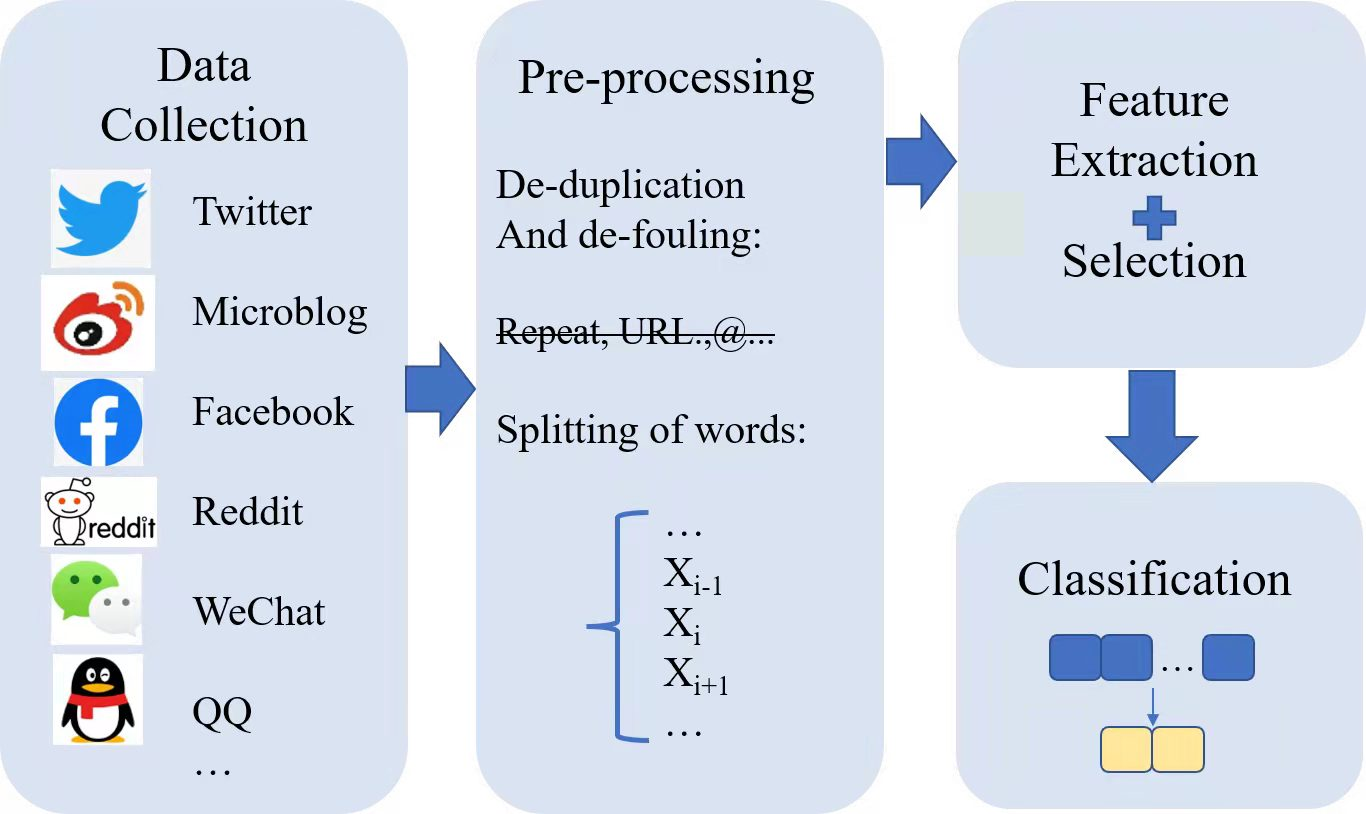
\includegraphics[width=0.8\linewidth]{figures/depression/text.png}		
	\caption{
	Flow chart of text-based depression recognition model.
	}
	\label{text}
\end{figure}

As shown in Fig \ref{text}, studies related to depression detection based on social media texts usually collect users' behavioral data on social network platforms such as Twitter, Weibo, Facebook, Reddit, or publicly published text content for analysis, while some other studies use relatively private social network data such as WeChat Moments and Qzone. Firstly, the raw data is pre-processed, such as removing other non-target language user data, removing deactivated words, URLs and special characters, etc., and then the sentences are divided into words. The next step is feature extraction and selection of the processed data. For the data selection and related feature engineering aspects, they can be mainly divided into the following aspects: linguistic features, behavioral features, emotional and cognitive features, demographic features, image features, etc. Finally, the attributes obtained by feature selection will be used to identify depressed users in social networks and to detect users with depression from normal users.

The researchers extracted features such as sentiment, mood and writing behavior of users from different social networking platforms and used various machine learning models for depression prediction.
The most applied traditional machine learning method is SVM~\cite{shing2018expert,smys2021analysis}, Peng~\cite{peng2019multi} et al. used a multi-core SVM model for depression identification based on social media data. aldarwish~\cite{aldarwish2017predicting} et al. used a plain Bayesian model , SVM models, etc. for depression rank identification and verified the utility of social media sites for depression rank identification. Secondly LR~\cite{eichstaedt2018facebook}, RF~\cite{tate2020predicting,kwakernaak2020using}, etc. are also widely used and Eichstaedt~\cite{eichstaedt2018facebook} et al. used LR methods to predict depressed users on Facebook. Finally, other classical machine learning classification algorithms such as NB, DT and XGBoost have also been used in related studies.

Deep learning methods are another approach that has been widely used by researchers in recent years. Among the frequently used methods are DNN, CNN, and RNN~\cite{yates2017depression,shen2017depression,orabi2018deep,ive2018hierarchical}.
Shen~\cite{shen2018cross} et al. proposed a cross-domain deep neural network model with feature adaptive transformation and combination strategy (DNN-FATC) to transfer relevant information to a heterogeneous domain, using sufficient Twitter data as the source domain and enhanced detection in some other target domain (e.g., Weibo).
Rao~\cite{rao2020mgl} et al. built a multilayer MGL-CNN to further identify depressed individuals in online forums by modeling them separately at sentence level and user level.
LSTM is a special type of RNN that learns long-term dependent information and has also been widely used in depression detection based on social media texts. Hu~\cite{hu2021depression} et al. proposed a Bi-LSTM-based depressive tendency detection model for microblog users. The content features of the microblog text were mined by bi-directional transmission and capturing the semantic dependencies of the context.

\subsubsection{Performance Comparison}
%\label{sec\_fquality}
%%%%%%%%%%%%%%%%%%%%%%%%%%%%%%%%%%%%%%%
.
\begin{table*}
\centering
\caption{Experimental results based on text}
\label{tab5}
\begin{tabular}{l|l|ll|lllll}

\hline
\multicolumn{1}{c|}{\multirow{2}{*}{ID}} & \multicolumn{1}{c|}{\multirow{2}{*}{Method}}                                          & \multicolumn{2}{c|}{Data}                                     & \multicolumn{5}{c}{Metrics}                                                                                                                        \\
\multicolumn{1}{c|}{}                    & \multicolumn{1}{c|}{}                                                                 & \multicolumn{1}{c}{Media}      & \multicolumn{1}{c|}{Dataset} & \multicolumn{1}{c}{Precision} & \multicolumn{1}{c}{Recall} & \multicolumn{1}{c}{F1-Score} & \multicolumn{1}{c}{Accuracy} & \multicolumn{1}{c}{AUC} \\
\hline
1                                       & SVM~\cite{de2013predicting}                                    & Twitter                        & -                           & 0.74                          & 0.63                       & -                            & 0.70                         & -                       \\
2                                       & Naïve Bayes~\cite{nadeem2016identifying}                       & Twitter                        & CLPsych 2015                & 0.82                          & 0.82                       & 0.81                         & 0.86                         & 0.94                    \\
3                                       & Logistic Regression~\cite{nadeem2016identifying}               & Twitter                        & CLPsych 2015                & 0.86                          & 0.82                       & 0.84                         & 0.82                         & 0.91                    \\
4                                       & Multi-kernel SVM~\cite{peng2019multi}                          & Weibo                          & -                           & 0.76                          & 0.77                       & 0.76                         & 0.83                         & -                       \\
5                                       & SVM+ Naïve Bayes~\cite{aldarwish2017predicting}                & Facebook, LiveJournal, Twitter & -                           & 1.00                          & 0.57                       & -                            & 0.63                         & -                       \\
6                                       & LDA(latent dirichlet allocation)~\cite{eichstaedt2018facebook} & Facebook                       & -                           & -                             & -                          & -                            & -                            & 0.72                    \\
7                                       & MGL-CNN~\cite{rao2020mgl}                                      & Reddit                         & RSDD                        & 0.63                          & 0.48                       & 0.54                         & -                            & -                       \\
8                                       & MGL-CNN~\cite{rao2020mgl}                                      & Online media                   & eRisk 2017                  & 0.63                          & 0.57                       & 0.60                         & -                            & -                       \\
9                                       & CNN~\cite{yates2017depression}                                 & Reddit                         & RSDD                        & 0.75                          & 0.57                       & 0.65                         & -                            & -                       \\
10                                      & MDL~\cite{shen2017depression}                                  & Twitter                        & -                           & 0.8+                          & 0.8+                       & 0.85                         & 0.8+                         & -                       \\
11                                      & DNN-FATC~\cite{shen2018cross}                                  & Twitter+ Weibo                 & -                           & -                             & -                          & 0.79                         & -                            & -                       \\
12                                      & CNNWithMax~\cite{orabi2018deep}                                & Twitter                        & CLPSych 2015                & 0.87                          & 0.87                       & 0.87                         & 0.88                         & 0.95                    \\
13                                      & MultiChannelCNN~\cite{orabi2018deep}                           & Facebook                       & Bell Let’s Talk             & 0.81                          & 0.84                       & 0.82                         & 0.83                         & 0.92                    \\
14                                      & Bi-LSTM~\cite{hu2021depression}                                & Weibo                          & -                           & -                             & -                          & -                            & 0.95                         & -                       \\
15                                      & LIWC~\cite{wolohan2018detecting}                               & Reddit                         & -                           & -                             & -                          & 0.68                         & 0.79                         & 0.75                   \\
\hline
\end{tabular}
\end{table*}

%%%%%%%%%%%%%%%%%%%%%%%%%%%%%%%%%%%%%%

Table\ref{tab5} summarizes the experimental results of the social platform text-based depression detection, including the source and name of the method, the type of data used and the source of the dataset (- indicates that the data used were collected by themselves), and the evaluation criteria of the experimental results including Precision, Recall, F1 Score, Accuracy, and AUC.


\ifx\allfiles\undefined
\input{tnnls\_suffix}
\fi 